\section{Event System and Knowledge Graph}
\label{sec:event-knowledge}

\subsection{Overview}
\label{sec:event-overview}

For the Knowledge Graph to build a picture of what is happening on the machine,
something has to watch and report. The Event System is that something: it
observes activity across the entire OS and feeds a continuous stream of
structured events into the graph, without any visible effect on the user and
without requiring applications to be rewritten for this platform.

Three sources feed into it, each covering a different slice of system activity.

\begin{table}[htbp]
\caption{Event sources and their coverage}
\label{tab:event-sources}
\begin{tabularx}{\linewidth}{lXX}
\toprule
\textbf{Source} & \textbf{App cooperation} & \textbf{What it sees} \\
\midrule
Kernel monitoring (eBPF) &
  None required &
  File opens, network connections, process lifecycle \\
Wayland compositor &
  Built-in (compositor is part of this project) &
  Window focus, app open/close, clipboard operations \\
First-party app events &
  Required; apps emit events directly &
  Rich semantic actions: document saved, search performed, tab opened \\
\bottomrule
\end{tabularx}
\end{table}

The design goal is baseline coverage for every app on the system without
requiring anything from third-party developers, combined with richer semantic
data where apps support it. eBPF provides the floor; structured app events
raise the ceiling.

\subsection{Kernel Monitoring with eBPF}
\label{sec:ebpf}

\emph{eBPF} (extended Berkeley Packet Filter) is a Linux kernel subsystem that
allows small, sandboxed programs to run inside the kernel without modifying
kernel source code or loading a kernel module~\cite{ebpf:io}. The name is
historical: the original Berkeley Packet Filter from 1992 was a mechanism for
filtering network packets; the \emph{extended} version, introduced in Linux
3.18 (2014) and substantially expanded in subsequent releases, is a
general-purpose in-kernel execution environment with applications far beyond
networking.

Before eBPF, the two main approaches to system monitoring were kernel modules
and \texttt{ptrace}. A kernel module runs with full kernel privileges and no
sandboxing; a bug in a module crashes the system. \texttt{ptrace} is a syscall
that allows one process to intercept the syscalls of another, but it introduces
substantial overhead and can only observe one process at a time. eBPF solves
both problems: programs are verified by the kernel's eBPF verifier before
loading (the verifier rejects any program that could loop infinitely, access
out-of-bounds memory, or crash the kernel), run at near-native speed via JIT
compilation, and can attach to hooks covering all processes on the system
simultaneously.

An eBPF program attaches to a specific kernel hook, called a \emph{tracepoint}
or \emph{kprobe}, and is executed each time the corresponding event fires: a
file being opened (\texttt{openat} syscall), a new process being created
(\texttt{clone}/\texttt{execve}), a network connection being established, and
so on. The program runs in kernel context, collects the relevant data (file
path, process ID, return value), and passes it to a user-space daemon via a
shared \emph{ring buffer} without the overhead of standard kernel I/O paths.
The result is a read-only window into every process on the machine with overhead
typically below 2\% of CPU time under normal desktop load.

At this layer, the system knows \emph{that} a process opened a file but not
\emph{why} or what it means to the user. That is intentional: eBPF provides the
universal baseline, and higher-level sources fill in the semantics where they
are available.

\paragraph{Why aya.}
Three libraries exist for writing eBPF programs from user space:
\texttt{libbpf}~\cite{libbpf}, \texttt{BCC} (BPF Compiler Collection), and
\texttt{aya}~\cite{aya}.

\texttt{libbpf} is the reference C library maintained in the Linux kernel tree.
It is stable and widely used, but integrating it into a Rust codebase requires
C FFI (Foreign Function Interface) bindings. Every call across the Rust/C
boundary requires \texttt{unsafe} blocks that the Rust compiler cannot verify,
partially defeating the purpose of writing the daemon in Rust.

\texttt{BCC} takes a different approach: eBPF programs are written as C strings
embedded in Python or Lua and compiled at runtime by LLVM on the target machine.
This makes BCC inappropriate for a production daemon: it requires LLVM to be
present on the user's system, compilation adds startup latency of several
seconds, and the Python runtime overhead is significant for a background service.

\texttt{aya} is a Rust-native eBPF library~\cite{aya}. Both the eBPF programs
(which run inside the kernel) and the user-space daemon are written in Rust.
Programs are compiled to eBPF bytecode at build time using \texttt{cargo}, not
at runtime, so no compiler is required on the end-user's machine. The result is
a fully Rust codebase with no unsafe FFI boundaries, no runtime compilation, and
no additional system dependencies beyond what the kernel already provides.

\paragraph{Noise filtering.}
eBPF can generate thousands of events per second under normal load, most of
which carry no useful information for the Knowledge Graph. Two filters in the
normalizer reduce this before events reach the bus. Identical operations on the
same file by the same process within 100 milliseconds are collapsed into a
single event with an updated timestamp. Paths under \texttt{/proc},
\texttt{/sys}, \texttt{/dev}, \texttt{/tmp}, and shared libraries under
\texttt{/usr/lib} are discarded entirely, since they have no semantic value in
a graph of user activity.

\subsection{Event Bus}
\label{sec:event-bus}

The Event Bus is a background daemon that receives events from all sources,
validates them against the event schema, and forwards them to registered
consumers. Its only job is to move and validate data; it does not interpret or
store anything. Figure~\ref{fig:event-flow} shows the full pipeline.

\begin{figure}[htbp]
\centering
\begin{tikzpicture}[
	src/.style={
		draw, thick, rectangle, rounded corners=3pt,
		minimum width=2.4cm, minimum height=0.8cm,
		font=\footnotesize, align=center, inner sep=4pt
	},
	proc/.style={
		draw, thick, rectangle,
		minimum width=2.4cm, minimum height=0.8cm,
		font=\footnotesize, align=center, inner sep=4pt
	},
	store/.style={
		draw, thick, cylinder, shape border rotate=90,
		minimum width=1.6cm, minimum height=1.0cm,
		font=\footnotesize, align=center, inner sep=4pt
	},
	arr/.style={->, thick},
	]
	
	% Sources (x=0)
	\node[src] (ebpf)    at (0, 4.5) {eBPF\\programs};
	\node[src] (wayland) at (0, 3.0) {Wayland\\compositor};
	\node[src] (apps)    at (0, 1.5) {First-party\\apps};
	\node[src] (journal) at (0, 0.0) {journald\\(known services)};
	
	% Pre-processors (x=3.6)
	\node[proc] (norm)   at (3.6, 4.5) {eBPF\\normalizer};
	\node[proc] (parser) at (3.6, 0.0) {Rule-based\\parser};
	
	% Event Bus (x=7.0) — tall box centered at y=2.25
	\node[proc, minimum width=2.2cm, minimum height=5.4cm, text width=1.8cm]
	(bus) at (7.0, 2.25) {Event Bus\\(Unix socket\\+ protobuf)};
	
	% Graph Writer (x=10.2), SQLite (x=12.8), Kuzu (x=12.8 lower)
	\node[proc]  (gw)     at (10.2, 2.25) {Graph\\Writer};
	\node[store] (sqlite) at (12.8, 3.6)  {SQLite\\(writes)};
	\node[store] (kuzu)   at (12.8, 0.9)  {Kuzu\\(queries)};
	\node[proc]  (promo)  at (10.2, -0.6) {Promotion\\pass};
	
	% Source arrows
	\draw[arr] (ebpf)    -- (norm);
	\draw[arr] (norm)    -- (bus.west |- norm);
	\draw[arr] (wayland) -- (bus.west |- wayland);
	\draw[arr] (apps)    -- (bus.west |- apps);
	\draw[arr] (journal) -- (parser);
	\draw[arr] (parser)  -- (bus.west |- parser);
	
	% Bus -> Writer -> SQLite, SQLite -> Promotion -> Kuzu
	\draw[arr] (bus.east) -- (gw);
	\draw[arr] (gw)       -- (sqlite);
	\draw[arr] (sqlite.south) -- (promo.east);
	\draw[arr] (promo)    -- (kuzu.south);
	
\end{tikzpicture}
\caption{Event pipeline. Raw kernel events pass through the eBPF normalizer
before reaching the bus. journald output from known system services passes
through a rule-based parser. First-party app events and compositor events
arrive already structured. All sources converge on the Event Bus, which
validates and forwards to the Graph Writer Daemon. The Graph Writer writes
to SQLite at full event throughput; a background promotion pass periodically
moves semantically valuable nodes into Kuzu for graph traversal queries.}
\label{fig:event-flow}
\end{figure}

\paragraph{Event schema.}
Every event, regardless of source, shares a common envelope. The identifier
uses \emph{UUID~v7}~\cite{rfc9562}, a variant of the universally unique
identifier standard introduced in RFC~9562 (2024). Unlike UUID~v4, which is
purely random, UUID~v7 embeds a millisecond-precision Unix timestamp in the
most significant bits. This makes UUIDs generated close together sort together
lexicographically, which matters for a time-series workload: inserting events
into the graph in roughly time order avoids the random-access write pattern
that UUID~v4 would produce and improves query performance for time-range
lookups. The envelope also carries a microsecond timestamp, a type label, a
source identifier, the originating process ID, and a session reference. The
type-specific data travels as a protobuf payload inside the envelope.

\begin{lstlisting}[language=C, caption={Common event envelope (protobuf)}]
message Event {
  string id         = 1;  // UUID v7 (time-sortable)
  string type       = 2;  // "file.opened", "window.focused", etc.
  int64  timestamp  = 3;  // microseconds since epoch
  string source     = 4;  // "ebpf", "wayland", "app:<id>"
  uint32 pid        = 5;  // originating process
  string session_id = 6;  // user session reference
  bytes  payload    = 7;  // type-specific protobuf message
}
\end{lstlisting}

A \texttt{file.opened} payload carries the file path, the application name,
and the operation flags. A \texttt{window.focused} payload carries the app ID
and window title. App events use a generic structure with a category, an
action, a subject, and an optional metadata map, which allows any first-party
application to emit meaningful events without requiring a dedicated payload
type per application.

Clipboard content is never logged. The bus records that a clipboard operation
occurred and its MIME type, not the content itself.

\paragraph{D-Bus coexistence.}
The custom Event Bus handles communication between project-internal components
only. D-Bus remains in place for everything it already handles: desktop
notifications, NetworkManager, Bluetooth, session management via
\texttt{systemd-logind}, sandboxed app portals, and standard third-party
applications. The two systems run in parallel with no overlap; nothing that
communicates over D-Bus today is changed.

\subsection{Write Architecture}
\label{sec:backpressure}

The Knowledge Graph has two structurally different workloads: a high-frequency
write path that must absorb thousands of eBPF events per second without
dropping data, and a query path that must traverse multi-hop graph
relationships efficiently for AI context and user queries. These two workloads
have conflicting requirements. A database optimized for one performs poorly at
the other. The write architecture addresses this by separating the two into
dedicated stores.

\paragraph{SQLite as the write store.}
All incoming events are written to \emph{SQLite}~\cite{sqlite}, a
battle-tested embedded relational database with excellent write throughput for
append-heavy workloads. SQLite is the write store: every event from every
source lands here first, at full throughput, with no analytical overhead.

The Graph Writer Daemon maintains a ring buffer of 10,000 event slots. A
batch write to SQLite is triggered by whichever threshold is reached first:
500 milliseconds have elapsed, or 1,000 events have accumulated. Both values
are configurable. When the buffer is full, the system works through three tiers
before discarding anything. First, it checks whether an identical event (same
type, source, and subject) already exists in the buffer and updates its
timestamp rather than inserting a duplicate. If no duplicate exists, it drops
the lowest-value event in the buffer, prioritizing raw eBPF read and write
events with no app-level context. Only if neither approach frees a slot is the
incoming event discarded, which should not occur under normal operating
conditions. Drop rates per tier are exposed as metrics and monitored by the
Anomaly Detector.

Raw eBPF events are retained in SQLite for 30 days and then discarded. They
serve the anomaly detection window and nothing else; they are never promoted
to Kuzu.

\paragraph{Kuzu as the query store.}
\emph{Kuzu}~\cite{kuzu} is the query store: an embedded graph database written
in C++ with first-class Rust bindings, released under the MIT license.
Embedded means it runs inside the Graph Daemon process with no separate server
process, no network port, and no additional service to manage. Kuzu uses
\emph{Cypher}~\cite{opencypher} as its query language, which is the interface
the AI daemon, first-party applications, and the FUSE timeline daemon all use
for graph traversal.

Kuzu operates on a curated graph, not a raw event log. Raw eBPF noise never
reaches it. Only semantically valuable nodes are promoted here: \texttt{File},
\texttt{App}, \texttt{Session}, \texttt{Project}, \texttt{UserAction}, and
their relationships. This keeps the Kuzu graph clean and traversal queries
fast.

\paragraph{Promotion pipeline.}
A background promotion pass runs periodically during idle periods, reading
from SQLite and writing promoted nodes and edges to Kuzu. The pass is
incremental: it tracks a high-water mark in SQLite and processes only new
records since the last run. Promotion criteria are deterministic: \texttt{Event}
nodes that have been correlated into \texttt{UserAction} clusters, \texttt{File}
nodes that have been accessed more than once, and all \texttt{Session} and
\texttt{Project} nodes are promoted. Single-occurrence raw eBPF events that
have not been correlated are not promoted.

The two stores have different query surfaces. SQLite answers time-range
lookups over recent raw events; Kuzu answers multi-hop graph traversals over
semantic history. The Graph Daemon presents a unified query interface to all
callers; the layer boundary is an implementation detail they never see.

\begin{lstlisting}[language=SQL, caption={Example Cypher query against Kuzu: files accessed last Tuesday}]
MATCH (f:File)-[:OPENED_BY]->(a:App)
WHERE f.last_modified > datetime('2026-03-01')
RETURN f.path, a.name
ORDER BY f.last_modified DESC
\end{lstlisting}

\subsection{Knowledge Graph}
\label{sec:knowledge-graph}

\paragraph{Why a graph.}
A relational database stores relationships as foreign keys across tables. A
graph database stores them as first-class edges. The difference is felt most
when querying across multiple entity types simultaneously: finding which files
a user worked on last Tuesday, which applications touched them, and whether any
of those applications are still running requires three joins and a subquery in
SQL and a single traversal in a graph. For an operating system where
everything is connected (processes open files, files belong to projects,
projects span sessions, sessions overlap with other applications), a graph
models the domain naturally.

The write architecture that feeds the graph is described in
Section~\ref{sec:backpressure}: SQLite absorbs the high-frequency event
stream, and a promotion pipeline moves semantically valuable data into Kuzu
for graph traversal. This section describes the Kuzu graph itself: its schema,
ingestion tiers, and the data that lives in it.

\paragraph{Schema.}
Figure~\ref{fig:kg-schema} shows the core node types and their relationships.
The schema is intentionally minimal at this stage; it will grow as the system
matures. \texttt{File}, \texttt{App}, \texttt{Session}, \texttt{Project},
\texttt{Event}, and \texttt{UserAction} are the primary entities. Every raw
occurrence from the event pipeline lands in SQLite first; promotion to Kuzu
happens after correlation into higher-level nodes. \texttt{UserAction} nodes
are derived abstractions built from clusters of related events and represent
meaningful activity rather than individual syscalls.

\paragraph{Event ingestion tiers.}
Not all event sources are equal in structure or volume, and the ingestion
strategy reflects that. Three tiers operate independently. All three write
to SQLite first via the write architecture described in
Section~\ref{sec:backpressure}; promotion to Kuzu follows asynchronously.

\emph{Tier~1: structured sources.} eBPF events, compositor events, and
first-party app events arrive already typed and schema-validated. They are
written to SQLite with no intermediate processing step. This tier handles
the large majority of writes and is the only tier with hard latency
requirements.

\emph{Tier~2: rule-based parsing.} journald output from known system services
(NetworkManager, bluetoothd, systemd-logind, and others) carries useful
structured information in a line-oriented format. A rule-based parser with
per-service patterns extracts this information synchronously. No machine
learning is involved; the patterns are deterministic and fast. Unknown services
and unmatched lines are discarded rather than approximated.

\emph{Tier~3: semantic enrichment (opt-in).} For document content specifically
--- PDFs opened in the viewer, browser page titles, text file contents --- a small
local model running at idle can extract topic labels and named entities and
attach them as properties on the corresponding \texttt{File} or \texttt{Event}
node. This is explicitly opt-in, runs only during idle periods, makes no
real-time promises, and is the only tier that involves a language model.
The appropriate model class is a sub-2B parameter instruction model
(Qwen2.5-1.5B or similar) that can run on CPU without saturating it; the
workload is low-frequency enrichment of user documents, not stream processing.
The graph is fully functional without this tier enabled.
The graph is fully functional without this tier enabled.

\begin{figure}[htbp]
\centering
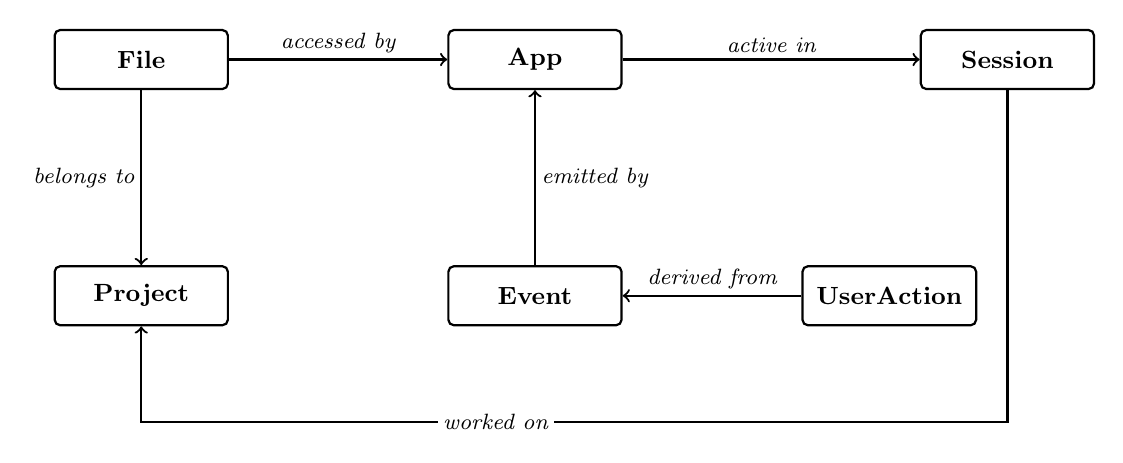
\begin{tikzpicture}[
	node/.style={
		draw, thick, rectangle, rounded corners=2pt,
		minimum width=2.2cm, minimum height=0.75cm,
		font=\small\bfseries, align=center, inner sep=5pt
	},
	edge/.style={->, thick},
	lbl/.style={font=\footnotesize\itshape, fill=white, inner sep=2pt},
	]
	
	\node[node] (file)    at (0, 4) {File};
	\node[node] (app)     at (5, 4) {App};
	\node[node] (session) at (11, 4) {Session};
	\node[node] (project) at (0, 1) {Project};
	\node[node] (event)   at (5, 1) {Event};
	\node[node] (action)  at (9.5, 1) {UserAction};
	
	\draw[edge] (file)   -- node[lbl, above] {accessed by}  (app);
	\draw[edge] (file)   -- node[lbl, left]  {belongs to}   (project);
	\draw[edge] (app)    -- node[lbl, above] {active in}    (session);
	\draw[edge] (event)  -- node[lbl, right] {emitted by}   (app);
	\draw[edge] (action) -- node[lbl, above] {derived from} (event);
	
	% Session -> Project: routed below all nodes
	\coordinate (sw) at (11, -0.6);
	\coordinate (se) at (0, -0.6);
	\draw[edge] (session.south) -- (sw) -- (se) -- (project.south);
	\node[lbl] at (4.5, -0.6) {worked on};
	
\end{tikzpicture}
\caption{Knowledge Graph core schema. Nodes represent entities; edges
represent relationships. \texttt{Event} nodes are the lowest-level entries,
created directly from the event pipeline. \texttt{UserAction} nodes are
derived abstractions built from clusters of raw events. A \texttt{File} can
belong to multiple \texttt{Project} nodes simultaneously; membership is an
edge, not a property of the file.}
\label{fig:kg-schema}
\end{figure}

\subsection{Project System}
\label{sec:projects}

A project is not a folder. It is a named context node in the Knowledge Graph
that groups related files, sessions, and activity across time and application
boundaries. The grouping is expressed as typed edges; a file does not carry a
project property, it participates in a \texttt{PART\_OF} relationship. This
means a file can belong to multiple projects simultaneously, and project
membership can be established, changed, or removed without touching the file
itself.

\paragraph{Philosophy: emergent, not prescribed.}
Projects are designed to arise from observed behavior and be confirmed by the
user, not to be created upfront and maintained manually. The graph accumulates
enough signal to infer that a coherent context exists; the user names and
confirms it. Both paths are available: explicit creation is supported for users
who prefer structure from the start, but it is not required.

\paragraph{The \texttt{.project} file.}
Every project can optionally carry a \texttt{.project} file at its root
directory. This is a TOML file that acts as the authoritative configuration for
that project and is the primary structured data source the Graph Daemon uses
when building the \texttt{Project} node. It is designed to be committed
alongside source code: a developer who clones a repository gets the project
context with it.

\begin{lstlisting}[language=bash, caption={Example .project file}]
[project]
name        = "CoffeeShop"
description = "Wii U homebrew mod manager"
status      = "active"   # active | paused | archived
created     = 2025-11-01
due         = 2026-06-01 # optional

[paths]
root    = "~/Repositories/coffeeshop"
include = [
    "~/Documents/coffeeshop-notes",
    "~/Downloads/wiiu-sdk-reference.pdf",
]
exclude = ["target/", "*.log"]

[git]
remote         = "https://github.com/timkicker/coffeeshop"
default_branch = "main"

[accounts]
github = "timkicker"

[links]
docs   = "https://wiiu.hacks.guide"
issues = "https://github.com/timkicker/coffeeshop/issues"

[tags]
values = ["cpp", "wiiu", "homebrew"]

[appearance]
accent_color = "#6aaa64"  # optional; overrides shell accent when focused

[focus]
suppress_notifications_from = ["steam", "discord"]

[modules]
active_when_focused = ["com.example.rust-waypointer"]

[ai]
context_scope = "project"  # minimal | project | time-scoped

[collaboration]
# Planned for a future release. The data model supports shared projects
# from the start; this field is reserved and currently ignored.
enabled = false
\end{lstlisting}

The \texttt{.project} file is the source of truth; the Graph Daemon reads it
at session start and whenever it changes on disk. Projects without a
\texttt{.project} file are fully supported: the node exists in the graph and
all features work, but configuration defaults apply and the project cannot be
distributed as a template.

\paragraph{Project node properties.}
The \texttt{Project} node in the graph carries the following properties, sourced
from the \texttt{.project} file where present and inferred or defaulted otherwise:
name, description, status, root path, creation timestamp, optional due date, tags,
and an accent color. The status field drives visibility across the system:
\texttt{active} projects appear prominently in Waypointer, the File Manager
sidebar, and AI context suggestions; \texttt{paused} projects are searchable
but not proactively surfaced; \texttt{archived} projects are read-only in the
graph and only reachable via explicit search. Archiving is a transition, not a
deletion: graph data is retained under the normal retention policy.

\paragraph{File membership and the \texttt{PART\_OF} edge.}
A file becomes part of a project through one of four mechanisms, in decreasing
order of specificity. First, explicit declaration in the \texttt{[paths]} block
of the \texttt{.project} file: any file under a declared include path is a
member. Second, rootdir heuristic: any file under the project root directory
is a candidate member, confirmed once the user has acknowledged the project.
Third, co-occurrence clustering: files that consistently appear together in the
same sessions, accessed by the same applications and terminal working directories,
are grouped as project candidates by a background inference pass. Fourth, manual
assignment via the File Manager or Waypointer: the user explicitly adds a file
to a project, which writes a \texttt{PART\_OF} edge directly.

A file can carry \texttt{PART\_OF} edges to multiple projects simultaneously.
The graph enforces no uniqueness constraint on this relationship.

\paragraph{Project-scoped AI context.}
When the AI access level is set to project-scoped (Level~2, described in
Section~\ref{sec:ai}), the \texttt{.project} file serves as the context seed
for the AI daemon. Name, description, tags, linked accounts, and recent
project activity from the graph are included in the context window before the
user's query. Waypointer surfaces project-specific quick actions when a project
is active: recent files, last commit message, open issues URL, and time spent
this week. These are graph queries, not hardcoded integrations.

\paragraph{Git integration.}
The presence of a \texttt{.git} directory in the project root is treated as a
strong project signal: the directory is automatically proposed as a project
root if no \texttt{.project} file exists. The current branch name is attached
as a property on the active \texttt{Session} node, providing context for
queries like ``what was I working on during the refactor branch last week.''
The \texttt{[git]} block in the \texttt{.project} file links the remote and
default branch for use in Waypointer quick actions and AI context.

Full git integration, covering commits as graph nodes, branch switches as
session context events, and pull request status as linked resources, is
planned for a subsequent release. The graph schema includes \texttt{Commit}
and \texttt{Branch} node types from the start so that this integration does
not require a schema migration when it arrives.

\paragraph{Project-aware system integrations.}
Projects are a cross-cutting concept and several system components integrate
with them directly. These integrations are described in detail in the
sections covering each component; the connections are summarized here for
reference.

The \emph{Focus Mode} (Section~\ref{sec:desktop}) is activated when the user
switches to a project context. It coordinates the shell accent color, Waypointer
search scope, File Manager root, terminal working directory, and notification
priority rules simultaneously.

The \emph{Health Daemon} (Section~\ref{sec:health}) tracks active focus time
per project from session data. This enables queries about work distribution
across projects and provides the signal for wellbeing observations such as
sustained single-project concentration over extended periods.

The \emph{Companion App} (Section~\ref{sec:companion}) uses the active project
as the Handoff context: switching away from the desktop surfaces the project's
linked resources, recent files, and notes on the phone.

The \emph{Module System} (Section~\ref{sec:modules}) supports the
\texttt{active\_when\_focused} manifest field, which activates a module only
when a specific project is in focus. A Rust-specific Waypointer provider that
surfaces \texttt{cargo} commands is the canonical example: it runs only when
the focused project carries the \texttt{rust} tag.

The \emph{Audit Log} (Section~\ref{sec:audit-log}) supports project-scoped
export: all activity records associated with a project within a specified date
range can be exported as a structured report. This is useful for time tracking,
client billing, and project handover.

\emph{Signed Profile Packages} (Section~\ref{sec:profiles}) can bundle
\texttt{.project} template files. An organization deploying a work profile
can pre-configure project structure, required accounts, AI scope restrictions,
and notification rules as part of the profile installation.

\paragraph{Automatic project inference.}
Project nodes in the graph are created explicitly when the user names a
project or a \texttt{.project} file is detected, but the graph also accumulates
enough signal to infer project membership without either. Files that
consistently appear together in the same sessions, terminal working directories
that recur alongside a fixed set of applications, and browser tabs that
co-occur with specific local files are all indicators that a coherent project
exists even without a name. A background inference pass groups these
co-occurrence clusters into candidate project nodes and presents them to the
user as suggestions rather than applying them automatically. The user can
confirm, rename, or dismiss each suggestion. Automatic inference is opt-in
and runs locally.

\subsection{Retention Policy}
\label{sec:retention}

The graph accumulates data indefinitely if left unchecked, which creates two
problems: storage grows, and the privacy surface area expands. The retention
policy defines how long data lives, with user control at every tier.

\begin{table}[htbp]
\caption{Knowledge Graph retention tiers}
\label{tab:retention}
\begin{tabularx}{\linewidth}{llX}
\toprule
\textbf{Tier} & \textbf{Default} & \textbf{Content} \\
\midrule
Raw eBPF events (SQLite) &
  30 days &
  High-volume, low-semantic-value syscall events. Retained for the
  anomaly detection window; never promoted to Kuzu and discarded
  after expiry. \\
Semantic nodes (Kuzu) &
  12 months rolling &
  File, App, Session, and NetworkConnection nodes promoted from SQLite.
  This is where AI query value lives. Nodes past the window
  are summarized rather than deleted. \\
Pinned nodes (Kuzu) &
  Permanent &
  Nodes explicitly marked by the user, active Project nodes, and nodes
  recently referenced in AI queries. Only manual deletion removes these. \\
\bottomrule
\end{tabularx}
\end{table}

\paragraph{Summarization.}
Hard deletion of aged nodes loses information abruptly. Instead, nodes past
the retention window are compacted into summary nodes that retain aggregate
statistics (access count, primary application, active period) while discarding
the individual event edges. The node still exists in the graph and AI queries
still find it; the granularity is reduced but the semantic content is
preserved. Summarization is triggered by access frequency rather than age: a
node that has not been queried in six months is a candidate regardless of when
it was created, while a node from two years ago that is queried regularly
remains granular. A background daemon identifies candidates nightly and
processes them during idle periods.

\paragraph{User controls.}
Settings exposes the retention window per tier with documented minimums, a
manual summarize-now option for specific time ranges, node and subgraph
deletion, full graph export for data portability, and storage usage broken down
by tier and time range. In managed deployments, administrators can set a
minimum retention for compliance-relevant audit events in a separate audit log,
but they cannot shorten the user's configured retention window for personal
graph data.

\subsection{Temporal Filesystem View}
\label{sec:temporal-fs}

The Knowledge Graph contains a complete record of which files were accessed,
created, and modified, when, and by which application. This makes it possible
to answer queries like ``show me everything I worked on last Tuesday'' without
relying on file modification timestamps, which applications regularly reset, or
on search indices, which do not capture access history.

The temporal filesystem view exposes this as a navigable virtual directory tree
via a \emph{FUSE} (Filesystem in Userspace) mount. FUSE is a Linux kernel
mechanism that allows a userspace process to implement a filesystem: the kernel
forwards directory listing and file open calls to the FUSE daemon, which
answers them from its own data source rather than from disk. The temporal view
mounts at \texttt{\textasciitilde/.timeline/} and is populated on demand by a
small daemon that translates directory traversal into Graph Daemon queries.

A path like \texttt{\textasciitilde/.timeline/2026-03-04/} lists all files the
user touched on that date, grouped by project where the graph has enough
context to determine project membership. The project grouping is deterministic
when a \texttt{.project} file is present and heuristic otherwise. Opening a
file through this path opens the actual file at its real location; the timeline
view is an index, not a copy. No additional storage is used.

\begin{lstlisting}[language=bash, caption={Temporal filesystem view examples}]
# List files worked on a specific date
ls ~/.timeline/2026-03-04/

# Browse by project across all time
ls ~/.timeline/projects/CoffeeShop/

# Files touched in the last week, grouped by project
ls ~/.timeline/last-7-days/

# Open a file as it appears in the timeline (opens real file)
xdg-open ~/.timeline/2026-03-04/CoffeeShop/report-draft.md
\end{lstlisting}

The FUSE daemon holds no persistent state of its own; every listing is a live
graph query. The mount is available only while the user session is active and
the Graph Daemon is running. It is read-only: files cannot be created, renamed,
or deleted through the timeline path.

A natural extension of the temporal view is causal chain visualization:
because the graph records not only which files were accessed but the sequence
and application context of those accesses, it is possible to reconstruct the
workflow that produced a given output. A query asking ``what did I do to produce
this file?'' can trace the chain of files opened, commands run, and applications
active in the session where the file was last modified. This is planned for a
subsequent release, built on the same FUSE and graph infrastructure described
here.
